% !TeX root = Protokoll.tex
\section{Gegengekoppelter Verstärker}

\FloatBarrier
\begin{figure}[!h]
\centering
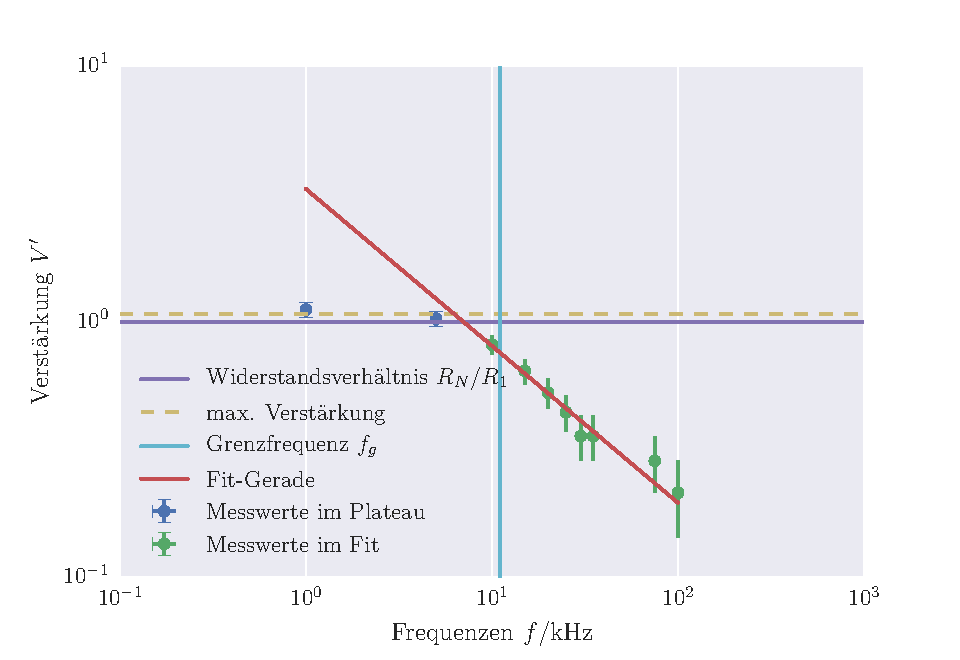
\includegraphics[scale=1]{../Grafiken/Gegengekoppelter_Verstaerker_1.pdf}
\caption{\label{fig:gegengekoppelter_verstaerker_1}}
\end{figure}
\FloatBarrier
\FloatBarrier
\begin{figure}[!h]
\centering
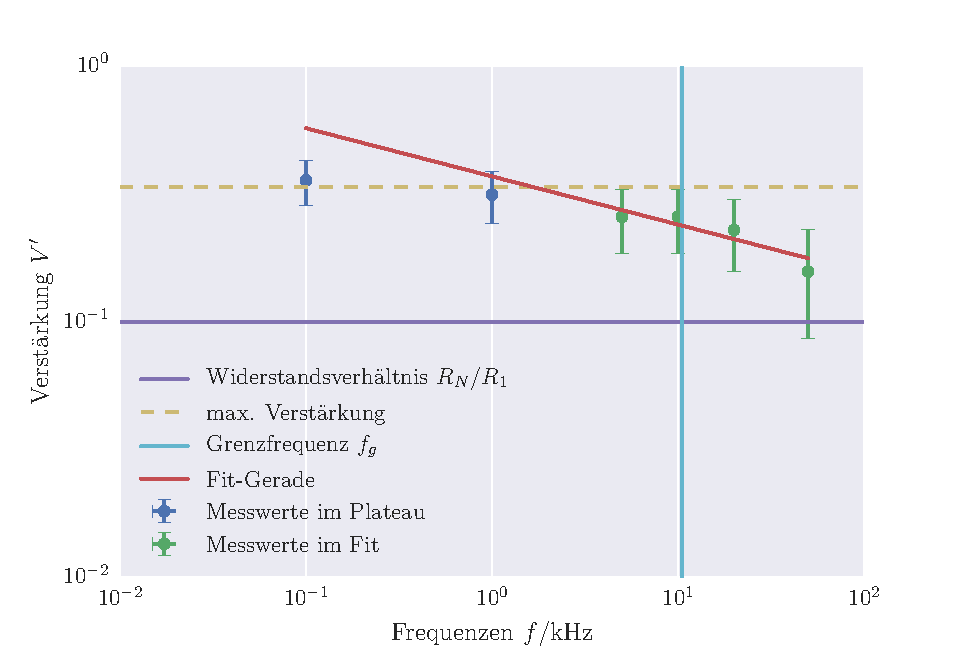
\includegraphics[scale=1]{../Grafiken/Gegengekoppelter_Verstaerker_2.pdf}
\caption{\label{fig:gegengekoppelter_verstaerker_2}}
\end{figure}
\FloatBarrier
\FloatBarrier
\begin{figure}[!h]
\centering
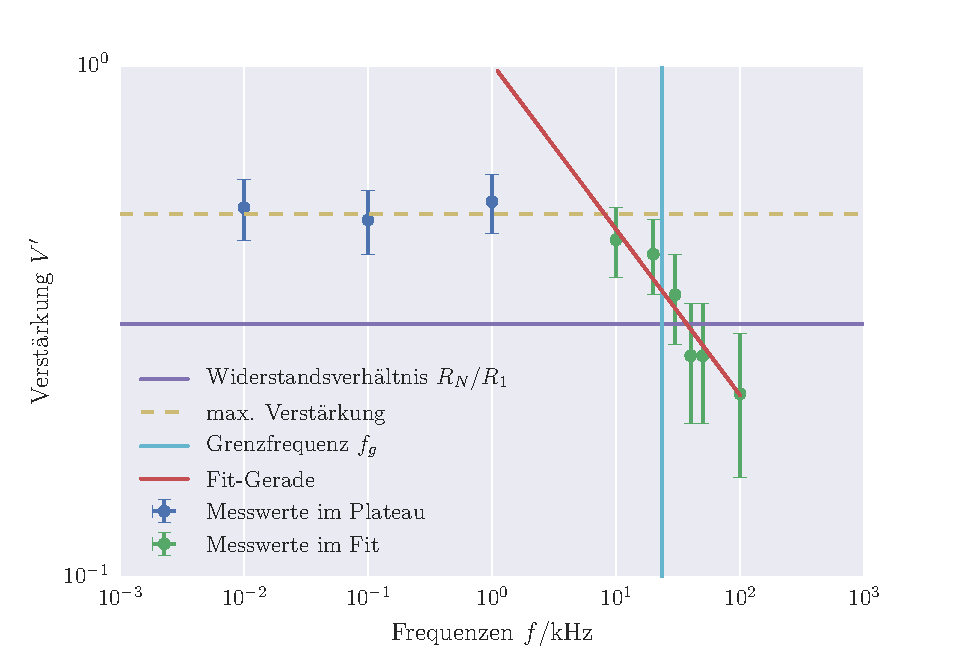
\includegraphics[scale=1]{../Grafiken/Gegengekoppelter_Verstaerker_3.pdf}
\caption{Doppellogarithmische Darstellung der Verstärkung der dritten gegengekoppelten Verstärkerschaltung in Abhängigkeit der Frequenz der Eingangsspannug. Zusätzlich wurden die Ausgleichsgerade
	durch die abfallenden Messwerte und eine senkrechte Gerade bei der Grenzfrequenz eingezeichnet. Ferner sind noch  zwei waagerechte Geraden dargestellt. Die eine markiert den Mittelwert der Messwerte im Plateau und die  andere
	den theoretischen Wert dieser Größe.\label{fig:gegengekoppelter_verstaerker_3}}
\end{figure}
\FloatBarrier
\FloatBarrier
\begin{figure}[!h]
\centering
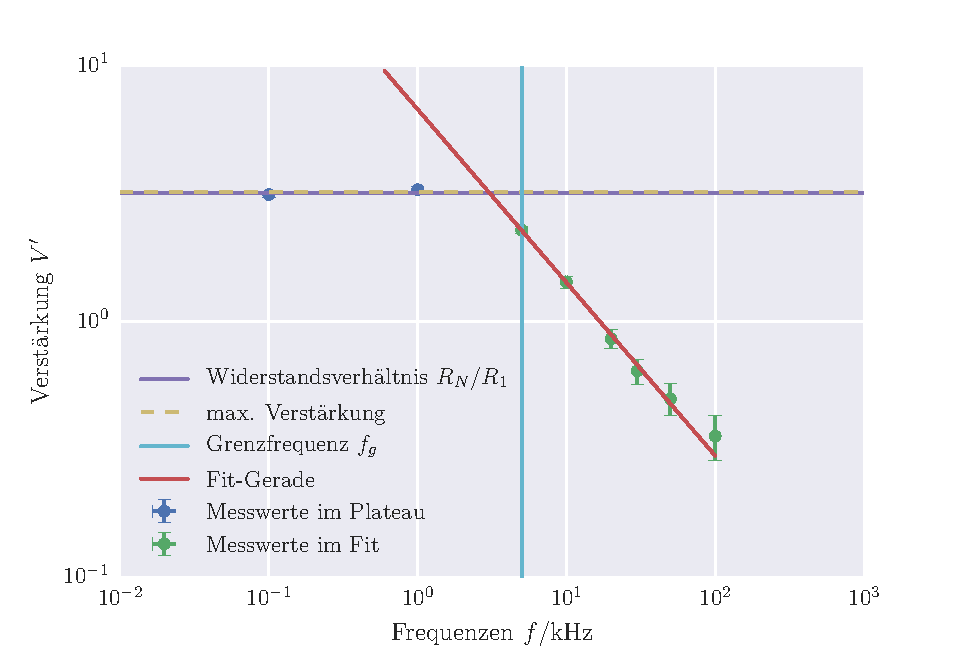
\includegraphics[scale=1]{../Grafiken/Gegengekoppelter_Verstaerker_4.pdf}
\caption{\label{fig:gegengekoppelter_verstaerker_4}}
\end{figure}
\FloatBarrier

\section{Amperemeter mit geringem Eingangswiderstand}

\section{Integrator- und Differentiatorschaltung}

\FloatBarrier
\begin{figure}[!h]
\centering
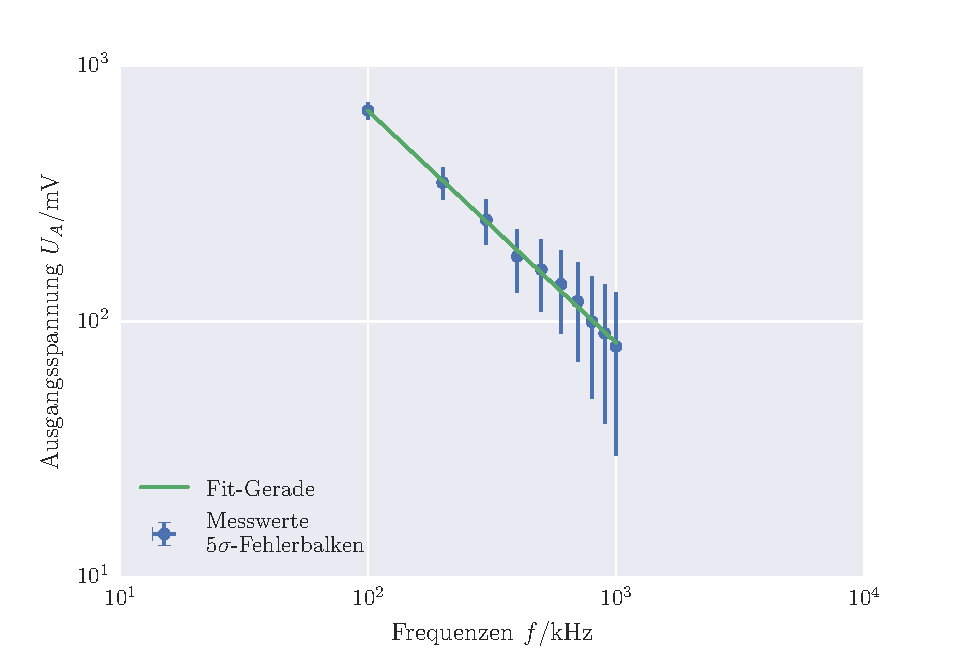
\includegraphics[scale=1]{../Grafiken/Integrator_Frequenz.pdf}
\caption{\label{fig:integrator_frequenz}}
\end{figure}
\FloatBarrier
\FloatBarrier
\begin{figure}[!h]
\centering
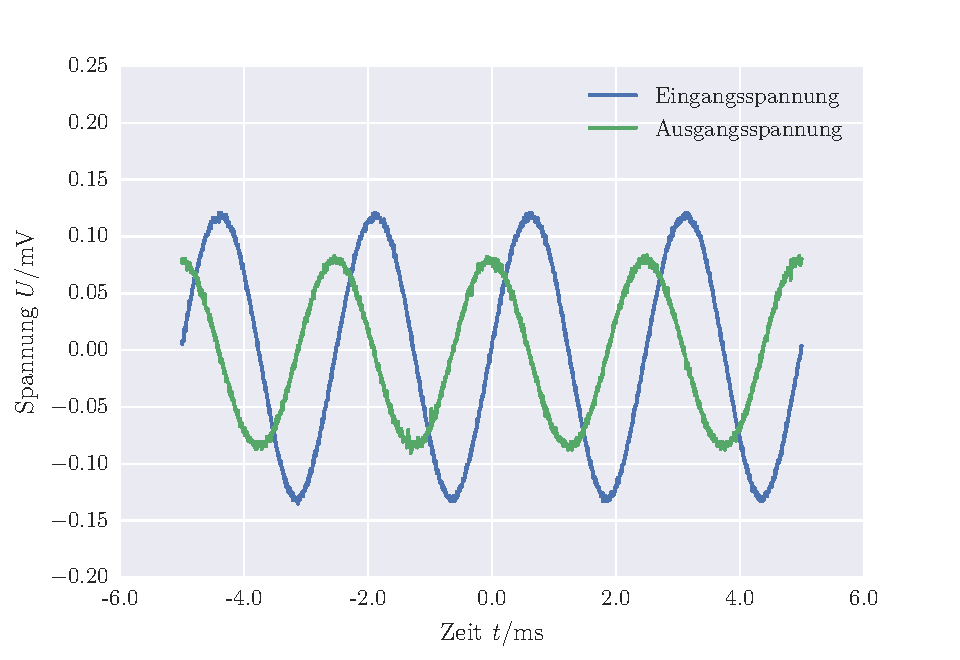
\includegraphics[scale=1]{../Grafiken/Integrator_Oszilloskop_Sinus.pdf}
\caption{Vom Oszilloskop aufgenommene Ein- und Ausgangsspannungen der Integratorschaltung. Auf dem Eingang
	liegt hier eine Sinusspannung. \label{fig:integrator_oszilloskop_sinus}}
\end{figure}
\FloatBarrier
\FloatBarrier
\begin{figure}[!h]
\centering
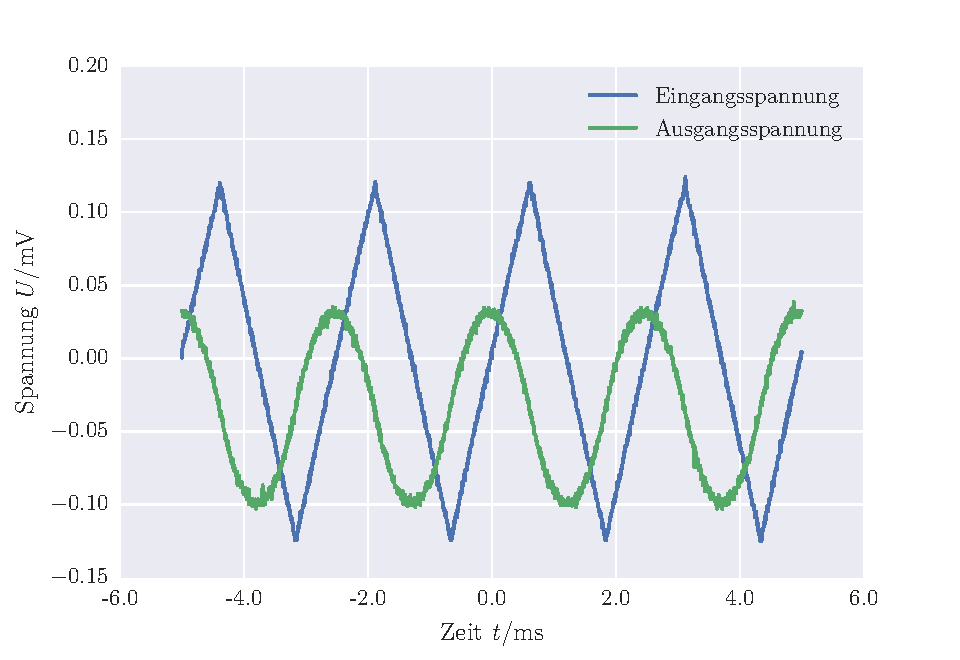
\includegraphics[scale=0.75]{../Grafiken/Integrator_Oszilloskop_Dreieck.pdf}
\caption{Vom Oszilloskop aufgenommene Ein- und Ausgangsspannungen der Integratorschaltung. Auf dem Eingang
	liegt hier eine Dreicksspannung. Die Ausgangsspannung in Parabelform entspricht dem theoretisch
	zu erwartendem Verlauf (periodische Abfolge nach oben respektive nach unten geöffneter 
	Parabeln).\label{fig:integrator_oszilloskop_dreieck}}
\end{figure}
\FloatBarrier
\FloatBarrier
\begin{figure}[!h]
\centering
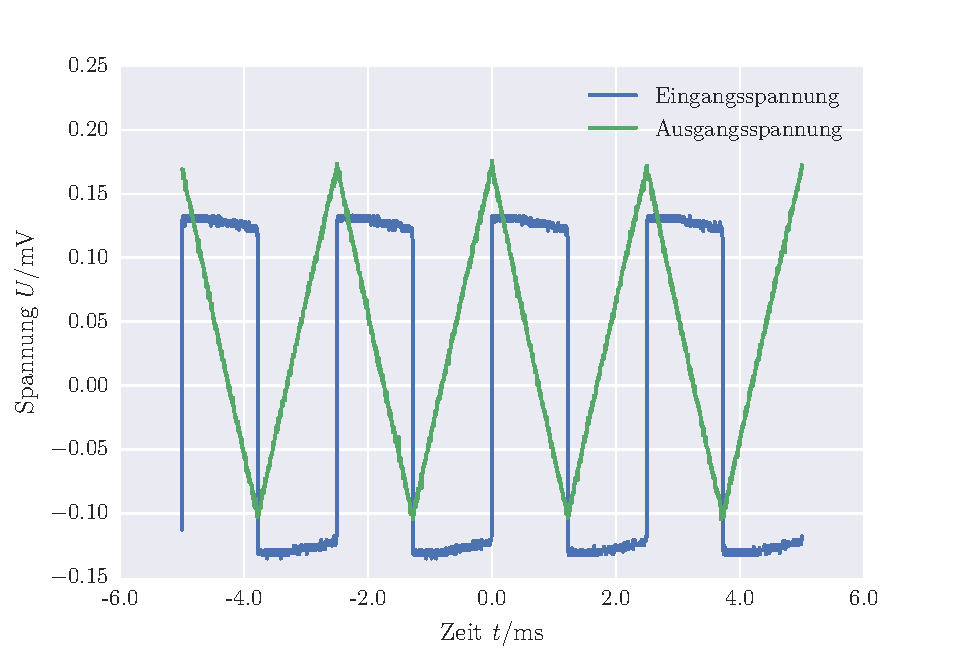
\includegraphics[scale=0.75]{../Grafiken/Integrator_Oszilloskop_Rechteck.pdf}
\caption{Vom Oszilloskop aufgenommene Ein- und Ausgangsspannungen der Integratorschaltung. Auf dem Eingang
	liegt hier eine Rechteckspannung.  Die Ausgangsspannung in Form einer Dreieckspannung entspricht dem theoretisch
	zu erwartendem Verlauf.\label{fig:integrator_oszilloskop_rechteck}}
\end{figure}
\FloatBarrier
\FloatBarrier
\begin{figure}[!h]
\centering
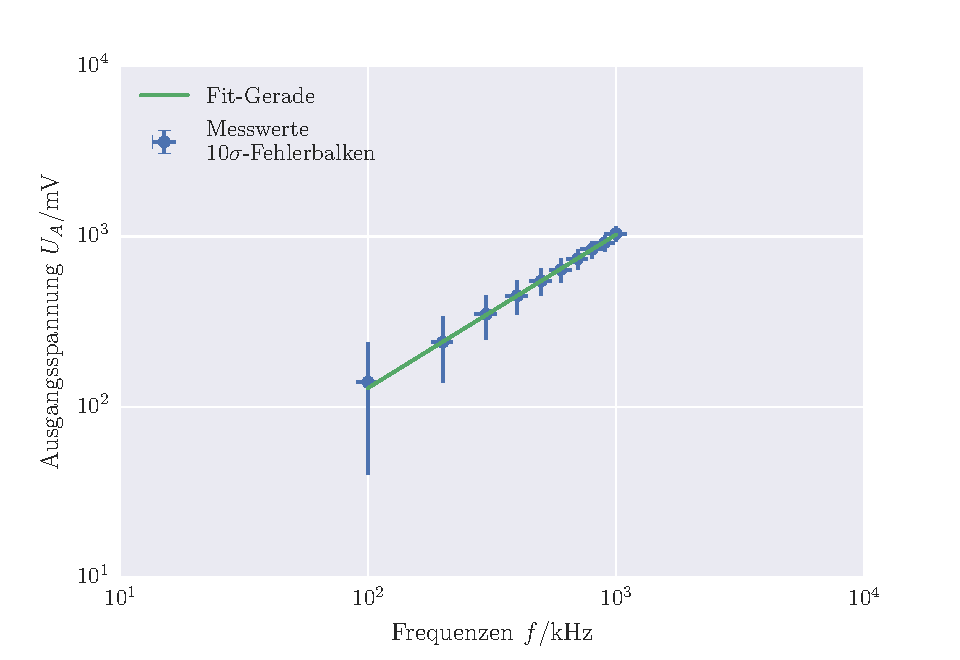
\includegraphics[scale=1]{../Grafiken/Differentiator_Frequenz.pdf}
\caption{\label{fig:differentiator_frequenz}}
\end{figure}
\FloatBarrier
\FloatBarrier
\begin{figure}[!h]
\centering
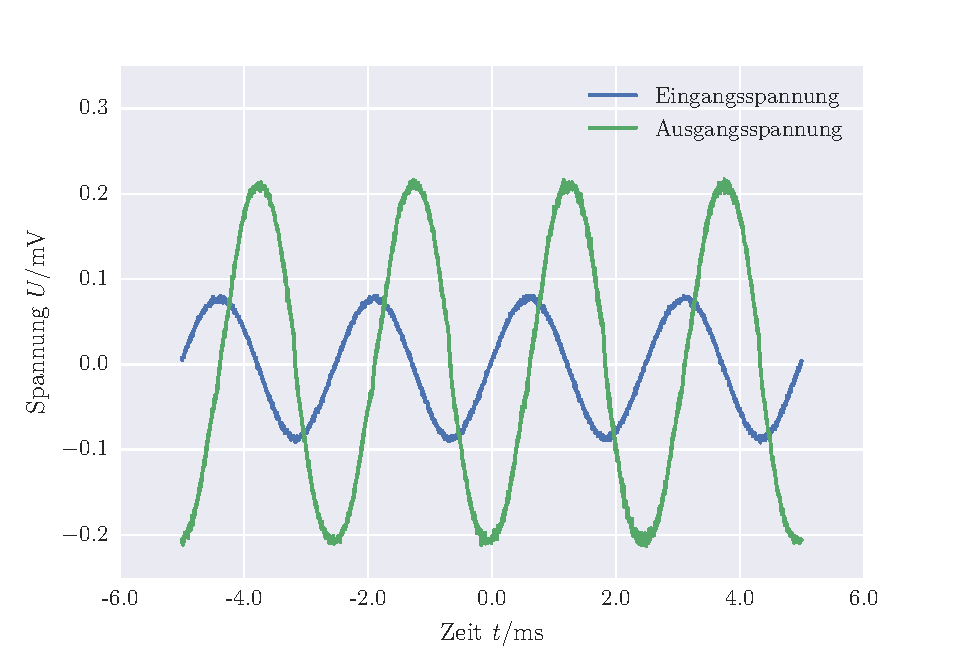
\includegraphics[scale=0.75]{../Grafiken/Differentiator_Oszilloskop_Sinus.pdf}
\caption{Vom Oszilloskop aufgenommene Ein- und Ausgangsspannungen der Differentiatorschaltung. Auf dem Eingang
	liegt hier eine Sinusspannung.\label{fig:differentiator_oszilloskop_sinus}}
\end{figure}
\FloatBarrier
\FloatBarrier
\begin{figure}[!h]
\centering
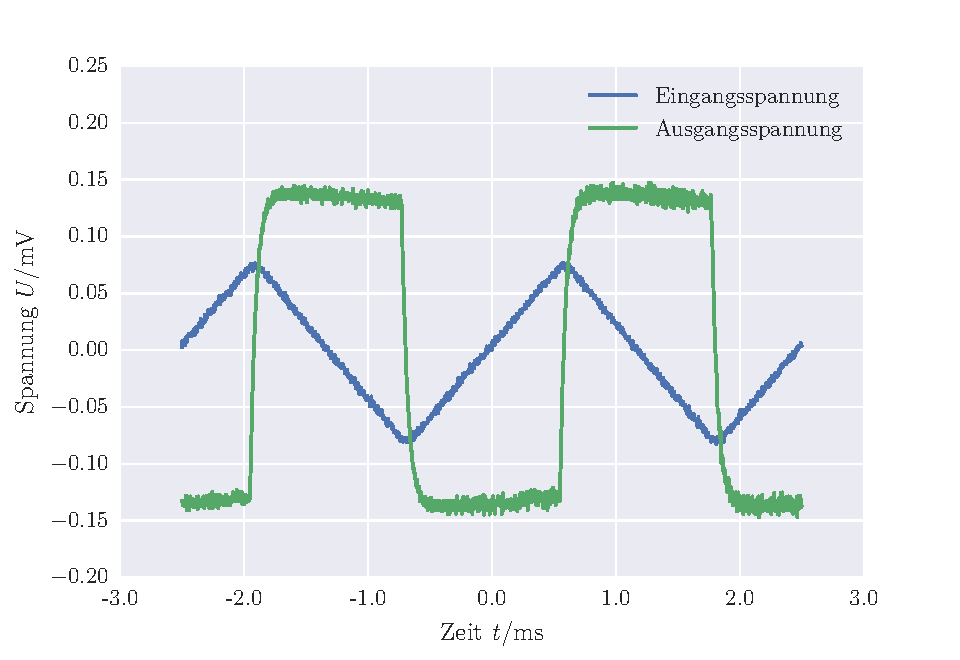
\includegraphics[scale=1]{../Grafiken/Differentiator_Oszilloskop_Dreieck.pdf}
\caption{\label{fig:differentiator_oszilloskop_dreieck}}
\end{figure}
\FloatBarrier
\FloatBarrier
\begin{figure}[!h]
\centering
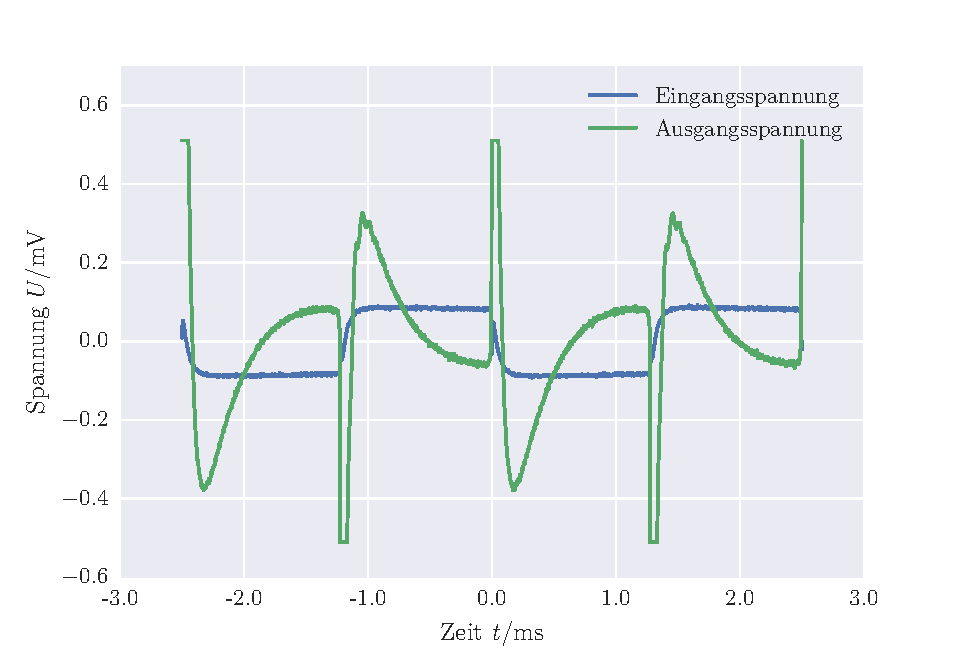
\includegraphics[scale=0.75]{../Grafiken/Differentiator_Oszilloskop_Rechteck.pdf}
\caption{Vom Oszilloskop aufgenommene Ein- und Ausgangsspannungen der Differentiatorschaltung. Auf dem Eingang
	liegt hier eine Rechteckspannung. Die Ausgangsspannung in Form schmalen hohen Peaks entspricht in etwa dem 
	theoretisch zu erwartendem Verlauf eines Delta-Kamms.\label{fig:differentiator_oszilloskop_rechteck}}
\end{figure}
\FloatBarrier

\section{Schmitt-Trigger}

\section{Funktionsgenerator}

\FloatBarrier
\begin{figure}[!h]
\centering
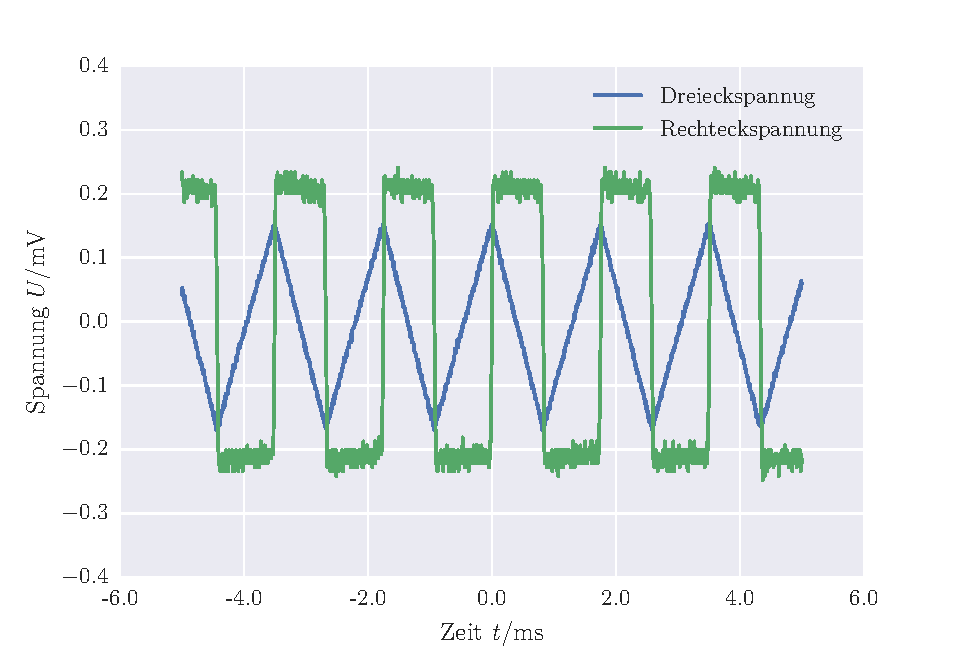
\includegraphics[scale=1]{../Grafiken/Funktionsgenerator.pdf}
\caption{Vom Oszilloskop aufgenommene Rechteck- und Dreiecksspannung der Funktionsgeneratorschaltung.\label{fig:funktionsgenerator}}
\end{figure}
\FloatBarrier

